\chapter{多器官功能障碍综合征和多器官功能衰竭}

\section{前沿学术综述}

多器官功能障碍综合征(multiple organ dysfunction
syndrome,MODS)是指机体遭受到严重感染、创伤、烧伤等严重打击后,两个或两个以上的器官同时或序贯性功能障碍。大量临床研究显示,器官障碍程度越重、器官障碍数目越多、患者病死率越高。若MODS发展为多器官功能衰竭(multiple
organ
failure,MOF),病死率可高达60%~94%,是严重感染、创伤和大手术后最常见的病死原因
\protect\hyperlink{text00007.htmlux5cux23ch1-6}{\textsuperscript{{[}1{]}}}
。急性器官障碍的数目和严重程度,明显影响患者的生活质量和病死率,多器官功能衰竭及MODS是当前重症医学所面临的最大挑战
\protect\hyperlink{text00007.htmlux5cux23ch2-6}{\textsuperscript{{[}2{]}}}
。

MODS的发病机制非常复杂。以往认为MODS是感染、创伤、烧伤等严重机体损伤难以遏制的直接后果。近20年的研究涉及到了MODS的病理生理学、病理学、免疫学、分子生物学以及分子流行病学,对MODS的认识逐步深刻。目前认为,MODS不仅与感染、创伤等直接损伤有关,在某种程度上,MODS与机体自身对感染、创伤的免疫炎症反应具有更为本质性的联系。也就是说,MODS的最大威胁来自失控的炎症反应
\protect\hyperlink{text00007.htmlux5cux23ch2-6}{\textsuperscript{{[}2{]}}}
。对机体炎症反应的深刻认识有利于早期认识MODS的病理生理紊乱,并使早期积极干预成为可能
\protect\hyperlink{text00007.htmlux5cux23ch3-6}{\textsuperscript{{[}3{]}}}
。MODS的发病机制提出了不少学说,但归纳起来主要包括炎症反应学说、自由基学说和肠道动力学说
\protect\hyperlink{text00007.htmlux5cux23ch2-6}{\textsuperscript{{[}2{]}}}
\textsuperscript{,}
\protect\hyperlink{text00007.htmlux5cux23ch4-6}{\textsuperscript{{[}4{]}}}
\textsuperscript{~}
\protect\hyperlink{text00007.htmlux5cux23ch6-6}{\textsuperscript{{[}6{]}}}
。炎症反应学说是MODS发病机制的基石。

根据MODS器官功能障碍发生的主要原因以及全身炎症反应综合征(systemic
inflammatory response
syndrome,SIRS)在器官功能损伤中的地位,可将MODS分为原发性MODS和继发性MODS。原发性MODS是指某种明确的损伤直接引起器官功能障碍,即器官功能障碍由损伤本身引起,在损伤早期出现,如严重创伤后,直接肺挫伤导致急性呼吸衰竭,横纹肌溶解导致肾脏功能衰竭,大量出血补液导致凝血功能异常等。在原发性MODS的发病和演进过程中,全身炎症反应综合征在器官功能障碍发生中所占比重较低。继发性MODS并非是损伤的直接后果,而与全身炎症反应综合征引起的自身性破坏关系密切,异常的炎症反应继发性造成远隔器官发生功能障碍。所以,继发性MODS与原发损伤之间存在一定的间歇期,易合并感染。在继发性MODS中,全身炎症反应综合征是器官功能损害的基础,全身性感染和器官功能损害是SIRS的后继过程。全身炎症反应综合征---全身性感染---MODS就构成一个连续体,继发性MODS是该连续体造成的严重后果
\protect\hyperlink{text00007.htmlux5cux23ch4-6}{\textsuperscript{{[}4{]}}}
\textsuperscript{,}
\protect\hyperlink{text00007.htmlux5cux23ch5-6}{\textsuperscript{{[}5{]}}}
。

近年的研究证实,免疫功能障碍不仅是MODS的重要组成部分,同时在MODS发生发展中发挥关键的作用。MODS免疫功能障碍包括机体过度或失控炎症反应和免疫功能麻痹的动态过程。免疫功能障碍发病机制复杂,多种因素交互促成。严重感染、创伤后机体免疫功能发生紊乱,既可能表现为亢进,也可能低下,且往往表现为早期炎症反应亢进,后期发生免疫功能抑制
\protect\hyperlink{text00007.htmlux5cux23ch6-6}{\textsuperscript{{[}6{]}}}
。

MODS涉及面广,临床表现复杂,但MODS具有以下显著特征:①发生功能障碍的器官往往是直接损伤器官的远隔器官;②从原发损伤到发生器官功能障碍在时间上有一定的间隔;③高排低阻的高动力状态是循环系统的特征;④高氧输送和氧利用障碍及内脏器官缺血缺氧,使氧供需矛盾尖锐;⑤持续高代谢状态和能源利用障碍。

所有MODS患者均应进入重症医学科治疗。尽管MODS的病因复杂、涉及的器官和系统多,治疗中往往面临很多矛盾,但MODS的治疗应遵循以下原则:

(1)积极治疗原发病 控制原发疾病是MODS治疗的关键,应重视原发疾病的处理。

(2)改善氧代谢,纠正组织缺氧 氧代谢障碍是MODS的特征之一,纠正组织缺氧是MODS重要的治疗目标。改善氧代谢障碍、纠正组织缺氧的主要手段包括增加全身氧输送、降低全身氧需、改善组织细胞利用氧的能力等。

(3)代谢支持与调理 MODS使患者处于高度应激状态,导致机体出现以高分解代谢为特征的代谢紊乱。器官及组织细胞的功能维护和组织修复有赖于细胞得到适当的营养底物,机体高分解代谢和外源性营养利用障碍,可导致或进一步加重器官功能障碍。因此,MODS时,代谢支持和调理的目标应当是减轻营养底物不足,防止细胞代谢紊乱,减少器官功能障碍的产生,促进组织修复。

(4)免疫调节治疗 免疫功能障碍、炎症反应失控是导致MODS的根本原因,免疫调控治疗、抑制全身炎症反应有可能阻断MODS的发展,最终可能降低MODS病死率。免疫调节治疗实际上就是MODS病因治疗的重要方向。

\section{临床问题}

\subsubsection{为什么要提出多器官功能障碍综合征的概念?}

多器官功能障碍综合征(MODS)的终末阶段是多器官功能衰竭。以MODS的概念代替多器官功能衰竭,反映了人们对多器官功能衰竭更为深入的认识和了解,将MODS定义为一个包括早期病理生理改变到终末期器官功能衰竭的连续的完整的病理生理过程,确立了动态和开放的MODS概念,为MODS的早期认识、早期诊断以及早期干预奠定了基础,具有重要的临床意义。

MODS概念的提出是认识进步的结果,但确定较为合理的MODS定义仍然困难。为了避免割裂MODS整个病理生理过程,美国胸科医师学会和美国危重病医学会提出了一个较为模糊的MODS定义,即各种疾病导致多个器官不能维持自身功能,从而影响全身内环境稳定性的状态。MODS表述的器官功能障碍可以是相对的,也可以是绝对的,而且器官功能障碍是动态的、连续的变化过程,对器官功能的动态观察必将有助于MODS的早期诊断和治疗。

\subsubsection{全身炎症反应综合征有何临床意义?}

1991年在芝加哥召开的美国胸科医师学会和危重病医学会联席会议,将感染或创伤引起的持续全身炎症反应失控的临床表现命名为全身炎症反应综合征,并制定了相应的诊断标准(表\ref{tab1-1})。全身炎症反应综合征可由感染因素引起,若进行性加重可导致全身性感染(systemic
infection或sepsis)、严重感染(severe
sepsis)、感染性休克,甚至多器官功能障碍综合征(MODS)。全身炎症反应综合征也可由创伤、烧伤、急性重症胰腺炎等非感染因素引起,进行性加重亦可引起MODS。全身炎症反应综合征是感染或非感染因素导致机体过度炎症反应的共同特征,MODS是全身炎症反应综合征进行性加重的最终后果。因此,就本质而言,全身炎症反应综合征是导致MODS的共同途径。

\begin{table}[htbp]
\centering
\caption{全身炎症反应综合征的诊断标准(符合下列两项或两项以上)}
\label{tab1-1}

\includegraphics[width=\textwidth,height=\textheight,keepaspectratio]{./images/Image00001.jpg}
\end{table}

尽管全身炎症反应综合征概念的提出是MODS认识上的重大进步,但全身炎症反应综合征的诊断标准本身存在许多不足,特别是把它作为一个综合征或疾病时,不能停留在诊断水平上,应积极寻找导致全身炎症反应综合征的致病因素。当然,我们也不能因为全身炎症反应综合征诊断标准存在问题而否认全身炎症反应综合征的重要意义。

\subsubsection{怎么认识多器官功能障碍综合征的病理生理机制?}

正常情况下,感染和组织创伤时,局部炎症反应对细菌清除和损伤组织修复都是必要的,具有保护性作用。当炎症反应异常放大或失控时,炎症反应对机体的作用从保护性转变为损害性,导致自身组织细胞死亡和器官衰竭。无论是感染性疾病(如严重感染、重症肺炎、急性重症胰腺炎后期),还是非感染性疾病(如创伤、烧伤、休克、急性胰腺炎早期等)均可能导致多器官功能障碍综合征(MODS)。可见,任何能够导致机体免疫炎症反应紊乱的疾病均可引起MODS。从本质上来看,MODS是机体炎症反应失控的结果。

感染、创伤是机体炎症反应的促发因素,而机体炎症反应的失控,最终导致机体自身性破坏,是MODS的根本原因。炎症细胞激活和炎症介质异常释放、组织缺氧和自由基、肠道屏障功能破坏和细菌和(或)毒素移位均是机体炎症反应失控的表现,构成了MODS炎症反应失控的3个互相重叠的发病机制学说------炎症反应学说、自由基学说和肠道动力学说(图\ref{fig1-1})。

\begin{figure}[!htbp]
 \centering
 
\includegraphics{./images/Image00002.jpg}
 \captionsetup{justification=centering}
 \caption{多器官功能障碍综合征的发病机制}
 \label{fig1-1}
  \end{figure} 

(1)炎症反应学说 炎症反应学说是MODS发病机制的基石。研究表明,感染或创伤引起的毒素释放和组织损伤并不是导致器官功能衰竭的直接原因,细菌和(或)毒素和组织损伤所诱发的全身炎症反应是导致器官功能衰竭的根本原因。

(2)缺血再灌注和自由基学说 缺血再灌注和自由基也是导致MODS的重要机制之一。MODS的自由基学说主要包括3方面:①氧输送不足导致组织细胞直接的缺血缺氧性损害;②缺血再灌注促发自由基大量释放;③白细胞与内皮细胞的互相作用,导致组织和器官损伤,最终发生MODS。从根本上来看,自由基学说也是炎症反应学说的重要组成部分。

(3)肠道动力学说 肠道动力学说的概念最早是由Meakins和Marshall提出的。肠道是机体最大的细菌和毒素库,肠道有可能是MODS患者菌血症的来源。另外,MODS患者菌血症的细菌往往与肠道菌群一致。因此,Meakins和Marshall提出肠道可能是MODS发生发展的动力器官(gut
motor)。在感染、创伤或休克时,即使没有细菌的移位,肠道内毒素的移位也将激活肠道及其相关的免疫炎症细胞,导致大量炎症介质的释放,参与MODS的发病。因此,肠道是炎症细胞激活、炎症介质释放的重要场地之一,也是炎症反应失控的策源地之一。从这一点来看,肠道动力学说实际上是炎症反应学说的一部分。

\subsubsection{全身炎症反应失衡怎样导致多器官功能障碍综合征的发生?}

基于全身炎症反应综合征是导致多器官功能障碍综合征(MODS)的根本原因这一认识,抑制全身炎症反应综合征有可能阻断炎症反应发展,最终可能降低MODS的病死率。20世纪90年代初期,大量的动物实验研究显示,抑制炎症介质能够明显降低感染或内毒素血症动物的病死率,这为临床MODS的救治带来希望。令人失望的是,内毒素单抗、肿瘤坏死因子α单抗等炎症介质拮抗剂在临床试验中相继失败,甚至个别研究报道增加病死率。由此迫使人们深入研究,并重新认识全身炎症反应综合征在MODS中的作用。

首先,引起注意的是机体受细菌毒素、损伤打击后,出现一过性细胞免疫功能降低,使机体对感染易感;其次,机体受细菌毒素、损伤刺激后,不仅释放炎症介质引起全身炎症反应综合征,同时大量释放内源性抗炎介质,后者可能是导致机体免疫功能损害的主要原因;第三,临床上盲目使用炎症介质拮抗剂,可能使免疫功能损伤加重,或许这就是炎症介质拮抗剂临床试验失败的主要原因。鉴于上述认识,1996年Bone针对感染或创伤时,导致机体免疫功能降低的内源性抗炎反应,提出了代偿性抗炎反应综合征(compensatory
anti-inflammatory response
syndrome,CARS)的概念。代偿性抗炎反应综合征作为全身炎症反应综合征的对立面,两者常常是不平衡的。如保持平衡,则内环境稳定得以维持,不会引起器官功能损伤。一旦全身炎症反应综合征和代偿性抗炎反应综合征失衡,将引起内环境失去稳定性,导致组织器官损伤,发生MODS
\protect\hyperlink{text00007.htmlux5cux23ch7-6}{\textsuperscript{{[}7{]}}}
\textsuperscript{,}
\protect\hyperlink{text00007.htmlux5cux23ch8-6}{\textsuperscript{{[}8{]}}}
。

如果把全身炎症反应综合征和代偿性抗炎反应综合征看作机体炎症反应天平的两端,则代偿性抗炎反应综合征作为天平的另一端,对全身炎症反应综合征发生、发展所起的关键性作用是不言而喻的。代偿性抗炎反应综合征的发生主要与抗炎性介质合成、抗炎性内分泌激素及炎症细胞凋亡等因素有关。

就其本质而言,MODS是全身炎症反应综合征和代偿性抗炎反应综合征免疫失衡的严重后果。全身炎症反应综合征和代偿性抗炎反应综合征失衡导致MODS的发展过程可分为3个阶段:①局限性炎症反应阶段,局部损伤或感染导致炎症介质在组织局部释放,诱导炎症细胞向局部聚集,促进病原微生物清除和组织修复,对机体发挥保护作用;②有限全身炎症反应阶段,少量炎症介质进入循环诱发全身炎症反应综合征,诱导巨噬细胞和血小板向局部聚集,同时,由于内源性抗炎介质释放增加导致代偿性抗炎反应综合征,使全身炎症反应综合征与代偿性抗炎反应综合征处于平衡状态,炎症反应仍属生理性,目的在于增强局部防御作用;③全身炎症反应综合征和代偿性抗炎反应综合征失衡阶段,表现为两个极端,一是大量炎症介质释放入循环,刺激炎症介质瀑布样释放,而内源性抗炎介质又不足以抵消其作用,导致全身炎症反应综合征;另一个极端是内源性抗炎介质释放过多而导致代偿性抗炎反应综合征。全身炎症反应综合征和代偿性抗炎反应综合征失衡的后果是炎症反应失控,使其由保护性作用转变为自身破坏性作用,不但损伤局部组织,同时打击远隔器官,导致MODS。

认识的进步,必然预示着在治疗上取得突破。恢复全身炎症反应综合征和代偿性抗炎反应综合征的动态平衡可能是MODS治疗的关键。

\subsubsection{多器官功能障碍综合征的二次打击学说有何临床意义?}

多器官功能障碍综合征(MODS)往往是多元性和序贯性损伤的结果,而不是单一打击的结果。1985年Dietch提出MODS的二次打击学说,将创伤、感染、烧伤、休克等早期直接损伤作为第一次打击,第一次打击所造成的组织器官损伤是轻微的,虽不足以引起明显的临床症状,但最为重要的是,早期损伤激活了机体免疫系统,尽管炎症反应的程度较轻,但炎症细胞已经被动员起来,处于预激活状态。此后,如病情稳定,则炎症反应逐渐缓解,损伤组织得以修复;如病情进展恶化或继发感染、休克等情况,则构成第二次或第三次打击。第二次打击使已处于预激活状态的机体免疫系统爆发性激活,大量炎症细胞活化、炎症介质释放,结果炎症反应失控,导致组织器官的致命性损害。第二次打击强度本身可能不如第一次打击,但导致炎症反应的爆发性激活,往往是致命性的(图\ref{fig1-2})。

\begin{figure}[!htbp]
 \centering
 
\includegraphics{./images/Image00003.jpg}
 \captionsetup{justification=centering}
 \caption{多器官功能障碍综合征的二次打击学说}
 \label{fig1-2}
  \end{figure} 

当第一打击强度足够大时,可直接强烈激活机体炎症反应,导致MODS,属于原发性MODS。但大多数患者MODS是多元性和序贯性损伤的结果,并不是单一打击的结果,这类MODS属于继发性MODS。常见的第二次打击包括继发性感染、休克、缺氧、缺血、创伤、手术等。对于多发性创伤的患者,如创伤严重,则直接可导致MODS,但多数患者经早期清创处理后基本稳定,而创伤早期发生的低血压导致各器官发生不同程度的缺血再灌注损伤及巨噬细胞、中性粒细胞激活,使患者出现发热、白细胞升高等炎症反应表现。创伤后3~7天,继发性感染或休克,使已处于预激活或激活状态的炎症细胞发生爆发性激活,结果使炎症反应失控,导致自身组织器官的损害,最终发展为MODS。

危重患者的病情往往是复杂的,机体遭受打击次数可能是两次,也可能是多次。多次反复打击将使机体炎症反应放大和失控更易发生,使患者更易发生MODS。另外,不仅机体免疫系统参与多次打击导致MODS的病理生理过程,凝血、纤溶、补体、激肽等多个系统均参与或累及。

MODS二次打击学说的提出,进一步强调了感染、创伤的后期处理。后期处理不当,其后果比早期损伤的结果更为严重,更具危害性。

\subsubsection{多器官功能障碍综合征有哪些临床特征?}

尽管多器官功能障碍综合征(MODS)的临床表现很复杂,但在很大程度上取决于器官受累的范围及损伤是由一次打击还是由多次打击所致。MODS临床表现的个体差异很大,一般情况下,MODS病程为14~21天,并经历4个阶段,包括休克、复苏、高分解代谢状态和器官衰竭阶段。每个阶段都有其典型的临床特征(表\ref{tab1-2}),且发展速度极快,患者可能死于MODS的任一阶段。

\begin{table}[htbp]
\centering
\caption{MODS的临床分期和特征}
\label{tab1-2}
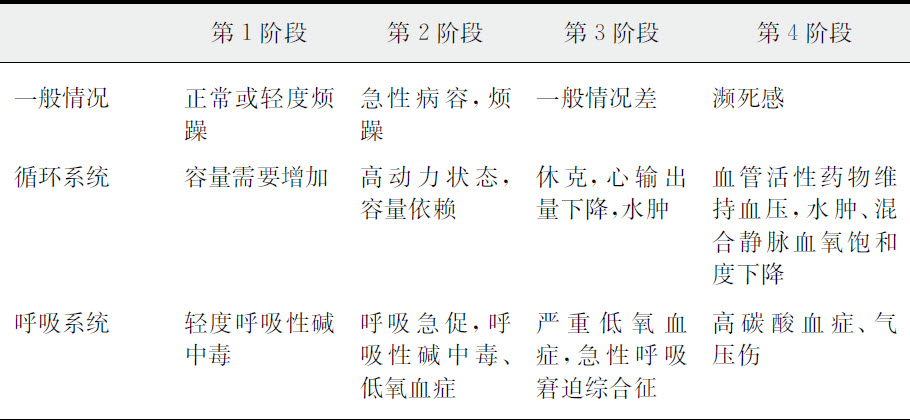
\includegraphics[width=\textwidth,height=\textheight,keepaspectratio]{./images/Image00004.jpg}
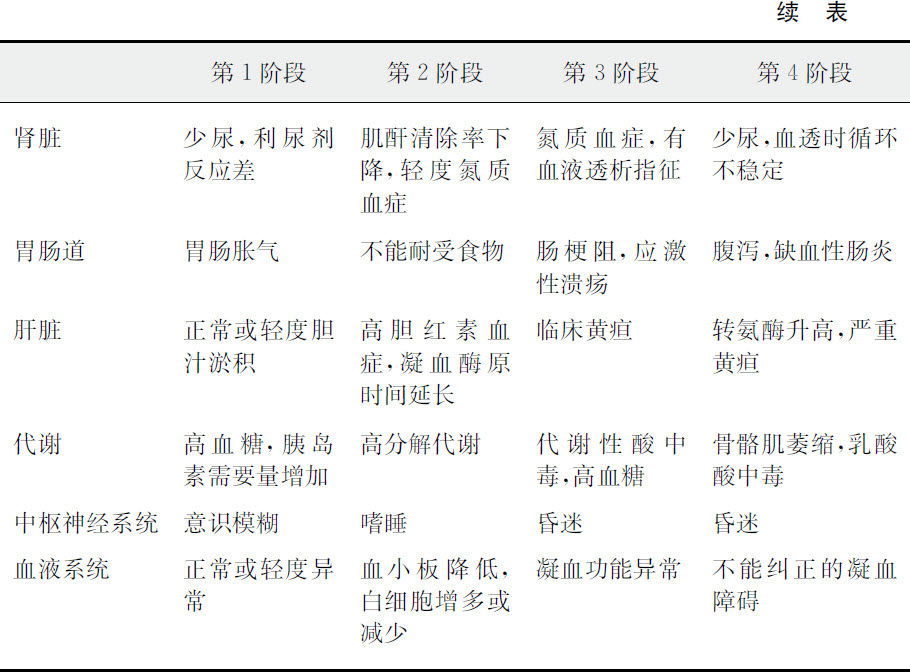
\includegraphics[width=\textwidth,height=\textheight,keepaspectratio]{./images/Image00005.jpg}
\end{table}



\subsubsection{不同多器官功能障碍综合征诊断标准有何差异?}

1980年Fry提出第一个多器官功能衰竭诊断标准。在此之前,循环、呼吸、肾脏和肝脏等器官已经具有单一器官衰竭的判断或诊断标准。应激性上消化道出血被认为是胃肠道功能衰竭。然而,血液、代谢和神经系统的衰竭或功能紊乱就缺乏明确的诊断方法。DIC显然是血液系统的功能紊乱,DIC诊断中除了出血等临床表现外,还需有血浆纤维蛋白降解产物水平升高。但血浆纤维蛋白降解产物浓度升高缺乏特异性,严重创伤或手术患者也可升高,使血液系统功能衰竭的诊断缺乏客观性。代谢紊乱是重症患者应激的结果,如果能够对代谢过程进行复杂的监测,则所有重症患者可能都存在所谓的“代谢障碍”,对代谢障碍的诊断缺乏可行性。神经系统功能障碍在重症患者中也很常见,但准确定量评价非常困难。另外,严重感染导致内脏器官严重损害时,往往血压和心输出量是正常或偏高的,直到出现休克或临终期,心血管系统才表现出功能衰竭。因此,Fry在提出多器官功能衰竭诊断标准时,仅包含了呼吸、肝脏、肾脏和胃肠道系统(表\ref{tab1-3})。

\begin{table}[htbp]
\centering
\caption{多器官功能衰竭诊断标准(Fry,1980年)}
\label{tab1-3}
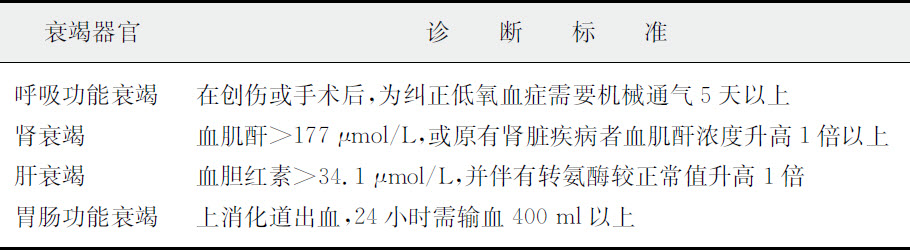
\includegraphics[width=\textwidth,height=\textheight,keepaspectratio]{./images/Image00006.jpg}
\end{table}

尽管Fry的多器官功能衰竭诊断标准是目前被公认的、应用最普遍的诊断标准,仍然存在很多问题:①该标准未包括神经系统、循环系统、血液系统等常见的器官功能衰竭;②以终末期的功能衰竭为诊断标准,不利于早期诊断和治疗;③难以反映多器官功能衰竭动态连续变化的病理生理过程;④呼吸功能衰竭的诊断过于严格,容易漏诊。

针对Fry诊断标准存在的问题,我们于1997年提出了修正的Fry-多器官功能障碍综合征(MODS)诊断标准(表\ref{tab1-4}),该标准结合国际常用的诊断标准,几乎包括了所有可能累及的器官或系统。当然,该标准未能包括MODS的整个病理生理过程,但避免了繁琐的程度评分,较为简捷,增加了临床实用性。

\begin{table}[htbp]
\centering
\caption{MODS诊断标准}
\label{tab1-4}
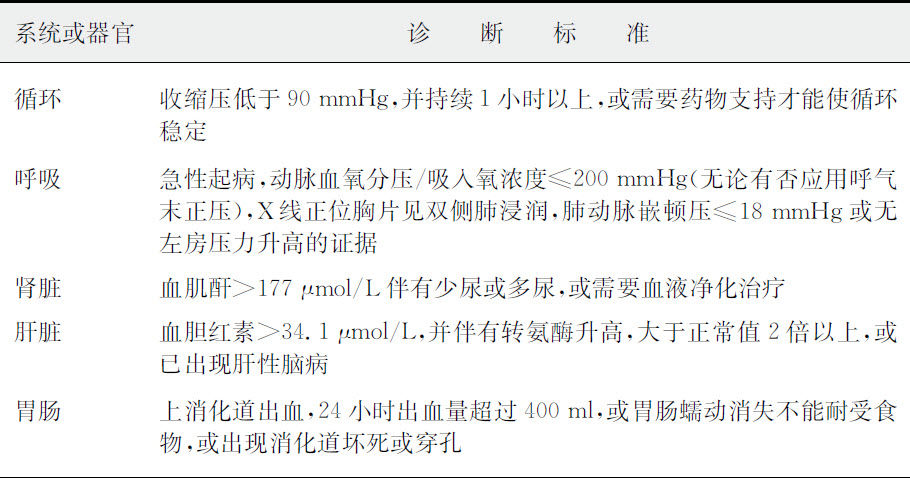
\includegraphics[width=\textwidth,height=\textheight,keepaspectratio]{./images/Image00007.jpg}
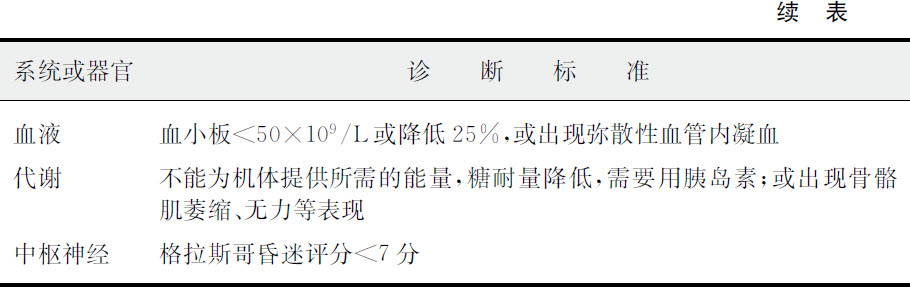
\includegraphics[width=\textwidth,height=\textheight,keepaspectratio]{./images/Image00008.jpg}
\end{table}

\subsubsection{哪些因素导致多器官功能障碍综合征的病死率增加?}

多器官功能障碍综合征(MODS)患者病死率高,认识病死危险因素,有助于早期确立MODS治疗对策。Knaus等学者对MODS的病死危险因素做了大规模的临床调查,概括了MODS病死的相关危险因素(表\ref{tab1-5})。\footnote{* APACHE:急性生理和慢性健康状况评分。}

\begin{table}[htbp]
\centering
\caption{MODS的病死危险因素}
\label{tab1-5}
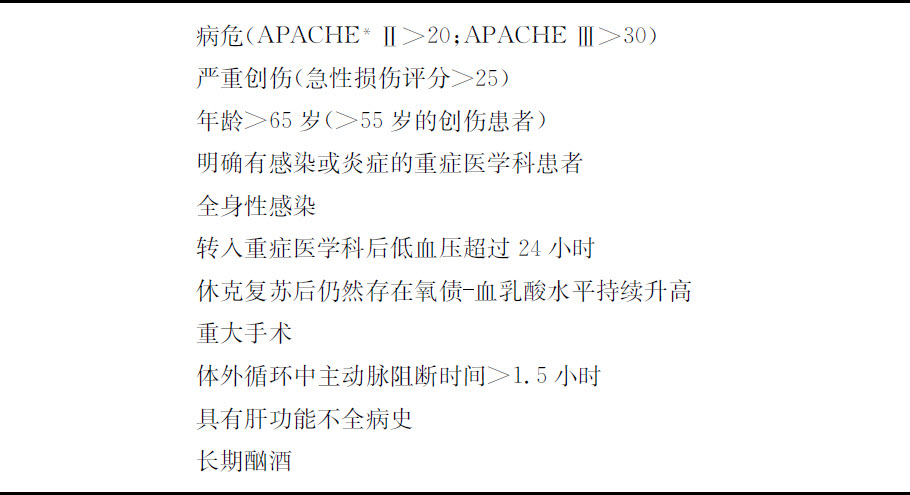
\includegraphics[width=\textwidth,height=\textheight,keepaspectratio]{./images/Image00009.jpg}
\end{table}

我国的研究也显示,免疫功能低下、转入ICU时的急性生理和既往健康评分(APACHE)Ⅱ评分、非手术、感染性休克及器官衰竭数目等因素与MODS患者死亡的关系显著。创伤、感染等MODS的病因、全身炎症反应综合征程度等因素与患者病死率无明显关系。

循环功能衰竭,即感染性休克为MODS最常见的直接病死原因;其次为中枢神经系统功能衰竭和心功能衰竭等,进一步提示在MODS治疗中,应特别注意纠正循环衰竭,并针对病因采取有效治疗措施,不应掉以轻心。

总之,MODS病死率依然很高,针对MODS病死危险因素进行积极处理和干预,可能是降低MODS病死率的关键。

\subsubsection{多器官功能障碍综合征时免疫功能障碍的基本概念是什么?}

免疫功能障碍不仅是多器官功能障碍综合征(MODS)的重要组成部分,同时在MODS发生发展中发挥关键的作用。MODS免疫功能障碍包括机体过度或失控炎症反应和免疫功能麻痹的动态过程。炎症反应本质上属于免疫反应的范畴,失控的炎症反应是MODS发生发展的根本机制,严重的炎症反应或细胞因子风暴可迅速引起微循环衰竭和感染性休克,继而发生DIC、呼吸衰竭和肝肾等器官功能障碍。免疫功能抑制可能与免疫效应细胞减少或功能抑制、机体呈调节T细胞或Th2极化和抗炎介质释放增多等因素有关。

临床免疫功能障碍可表现为多器官功能障碍,可于数小时、数天或数周发病,病程也长短不一。如爆发型流脑、中毒性休克综合征及严重猪链球菌Ⅱ型感染等严重炎症反应常在很短的时间内迅速发生休克、呼吸衰竭、肾衰竭和DIC等。免疫功能抑制患者常表现为原发感染难以痊愈,潜在感染的复发,或出现新的继发性感染。目前准确定量评价机体炎症反应水平和免疫功能紊乱性质、程度仍存在困难,还缺乏准确的临床判断指标和诊断方法。通过仔细的临床观察和密切的实验室检测,早期诊断器官功能损害或衰竭,并给予强化的器官功能支持治疗,能够避免部分患者死于继发性器官功能衰竭。

尽管MODS中免疫功能衰竭日益受到重视,然而由于其功能复杂性,免疫功能障碍缺乏明确的定义,亦无公认的临床判断指标。对免疫复杂而精细调节的反应和机制进行研究,从而充分发挥机体的防御作用,对减少损伤、促进机体康复是非常必要的。

\subsubsection{哪些是多器官功能障碍综合征时合并免疫功能障碍的主要病因?}

(1)感染 全身性感染(sepsis)是临床上引起免疫功能障碍常见的原因,如肺部感染、腹腔感染、血流感染、尿路感染及皮肤感染等。爆发型流脑、严重猪链球菌Ⅱ型感染及某些类型链球菌、葡萄球菌感染所致中毒性休克综合征等也是临床常见的免疫功能紊乱性疾病。

(2)创伤、烧伤、手术 许多非感染因素如严重创伤、大手术等也可以活化炎细胞,如变性坏死的组织细胞及其产物、缺氧、免疫复合物等。有研究证实,创伤程度越重,机体免疫抑制效应越强,表现为单核细胞功能降低、淋巴细胞增殖受到抑制、白介素-2合成减少等,继发感染并发症是导致伤员死亡的主要原因之一。

(3)急性胰腺炎 胰腺细胞受损首先导致局部炎症反应,细胞因子进入血液循环可致白细胞激活,引发全身炎症反应综合征和多器官功能障碍综合征(MODS)。重症急性胰腺炎可在数小时或数天病情迅速加重,甚至在早期发生MODS而危及生命。

(4)营养不良 临床研究表明,危重病人营养不良的发生迅速而普遍,且营养不良本身已成为预测危重症预后不良风险的重要因素。由于营养素摄入不足、消耗增加或代谢异常等导致机体营养不良,引起胸腺和淋巴组织早期就受到损害,致使免疫功能低下,容易并发各种感染。

(5)免疫性疾病 免疫组织、细胞或分子存在结构、数量或功能缺陷,导致免疫防御功能损害,表现为抗感染能力下降,易发生反复或持续感染,如白细胞减少症、粒细胞缺乏症。

(6)其他疾病 如慢性消耗性疾病、恶性肿瘤等。最近研究发现脑卒中诱导的免疫抑制(stroke-induced
immunosuppression)可导致卒中后感染并发症增加
\protect\hyperlink{text00007.htmlux5cux23ch9-6}{\textsuperscript{{[}9{]}}}
。

(7)医源性因素 某些药物如免疫抑制剂、化疗药物、放疗等可显著抑制机体免疫功能。

\subsubsection{多器官功能障碍综合征免疫功能障碍的发病机制是什么?}

免疫功能障碍发病机制复杂,多种因素交互促成,且有待深入研究。严重感染、创伤后机体免疫功能发生紊乱,既可能表现为亢进,也可能低下,且往往表现为早期炎症反应亢进,后期发生免疫功能抑制
\protect\hyperlink{text00007.htmlux5cux23ch10-6}{\textsuperscript{{[}10{]}}}
。

(1)早期炎症反应亢进 炎症反应与免疫反应关系密切。遇到损伤信号后,机体吞噬细胞、NK细胞等迅速动员,执行防卫功能,吞噬、杀伤或抑制细菌或其他小颗粒,如果被吞噬的颗粒较大,吞噬细胞无法将其包围,或细胞损伤崩解,则颗粒内容物将逸出而损伤邻近正常组织。

严重感染、创伤早期,各种免疫细胞和多种体液因子参与早期炎症反应,吞噬细胞如中性粒细胞、单核细胞和巨噬细胞等活化,补体系统激活。活化的炎细胞释放的炎症介质一般在局部发挥防御作用,血浆中一般测不出炎症介质。全身炎症反应综合征时,大量炎细胞活化,分泌的炎症介质溢出到血浆中。炎症时细胞因子往往呈序贯性表达和不同幅度的升高,大量释放的炎症因子、毒素、蛋白酶导致组织细胞损伤。随着病情好转,血浆中炎症介质减少。在爆发型流脑、中毒性休克综合征、严重猪链球菌Ⅱ型感染及急性爆发型胰腺炎等,引起严重的炎症反应或暴风式炎症反应(细胞因子风暴),很短的时间内剧烈的炎症反应迅速引起休克和多器官功能障碍综合征
\protect\hyperlink{text00007.htmlux5cux23ch11-6}{\textsuperscript{{[}11{]}}}
\textsuperscript{,}
\protect\hyperlink{text00007.htmlux5cux23ch12-6}{\textsuperscript{{[}12{]}}}
。

(2)免疫功能抑制 免疫功能抑制又称免疫麻痹(immunoparalysis),常引起机体继发感染,甚至因严重感染而死亡,其发病机制复杂,可能与以下因素有关。

吞噬细胞减少或功能抑制,重症患者往往因为高血糖、应用免疫抑制剂、放化疗等引起白细胞减少、粒细胞缺乏等。

树突状细胞减少或功能抑制,树突状细胞数量减少参与全身性感染免疫抑制发生。研究观察到,全身性感染小鼠3天发现脾脏树突状细胞数量明显减少。临床研究也观察到,严重感染和感染性休克的患者循环髓系树突状细胞和浆细胞样树突状细胞均明显减少
\protect\hyperlink{text00007.htmlux5cux23ch13-6}{\textsuperscript{{[}13{]}}}
\textsuperscript{,}
\protect\hyperlink{text00007.htmlux5cux23ch14-6}{\textsuperscript{{[}14{]}}}
。树突状细胞的抗原提呈能力降低与免疫抑制也有关。Poehlmann等观察到,存在免疫麻痹的严重感染和感染性休克患者,循环髓系树突状细胞和浆细胞样树突状细胞均明显减少,人类白细胞相关抗原-DR表达明显降低,且至28天仍低于正常。Kawasaki等也证实在创伤后小鼠脾脏树突状细胞的抗原提呈能力明显下降。

免疫效应细胞减少:严重感染和感染性休克患者免疫效应细胞减少参与免疫抑制。Hotchkiss等观察到,对严重感染及感染性休克死亡的患者行尸检发现脾脏CD4\textsuperscript{+}
T细胞和B细胞显著减少,且这些免疫效应细胞明显减少主要系细胞凋亡所致。在重症医学科中因严重感染死亡的患儿尸检结果同样证实脾脏CD4\textsuperscript{+}
T细胞和B细胞显著减少。上述研究提示免疫效应细胞大量丢失介导免疫抑制发生。

负性免疫调节细胞增多:机体内调节T细胞发挥负性免疫调控效应。研究发现,合并免疫麻痹的感染性休克患者病程第1~2天,外周血调节T细胞绝对数和相对比例均即明显升高,第3~6天进一步增加,与存活组相比,死亡组患者调节T细胞持续升高。提示调节T细胞可能与免疫抑制有关。

细胞因子表达谱改变:全身性感染病程中细胞因子分泌异常也与免疫抑制相关。Kawasaki等发现创伤后小鼠脾脏树突状细胞分泌白介素-12明显减少。Wen等研究显示,盲肠结扎穿孔小鼠脾脏白介素-12均明显降低,而抗炎细胞因子白介素-10则明显升高。说明细胞因子谱表达异常参与全身性感染的免疫抑制发生。

\subsubsection{多器官功能障碍综合征免疫功能障碍的病理改变有哪些表现?}

免疫功能障碍患者免疫器官可出现各种类型、程度不一的病理改变。

炎症反应主要是机体对损伤或感染的防御反应,以变质、渗出和增生为基本病理特征。脏器损害复杂多样,病变程度轻重不一,可出现某一个或多个脏器突出损害表现。组织可仅轻微的炎症反应,也可呈现明显的白细胞浸润。

免疫抑制患者的免疫器官可出现明显异常。有研究观察到,严重感染及感染性休克患者脾脏大量CD4\textsuperscript{+}
T细胞和B细胞凋亡,而CD8\textsuperscript{+}
T细胞、自然杀伤细胞和巨噬细胞无明显变化。另有研究发现,全身炎症反应综合征患者中性粒细胞往往表现为凋亡延迟,生存周期的延长,造成过度的炎症反应而损伤组织
\protect\hyperlink{text00007.htmlux5cux23ch15-6}{\textsuperscript{{[}15{]}}}
\textsuperscript{,}
\protect\hyperlink{text00007.htmlux5cux23ch16-6}{\textsuperscript{{[}16{]}}}
。

\subsubsection{多器官功能障碍综合征免疫功能障碍的病理生理改变特点是什么?}

多器官功能障碍综合征(MODS)免疫功能障碍包括机体过度或失控炎症反应和免疫功能麻痹的动态过程。由于众多细胞因子和体液介质的复杂作用,引起一系列复杂的病理生理改变,严重威胁患者生命。

炎症反应主要是机体对损伤或感染的防御反应。炎症细胞聚集和激活可释放各种蛋白酶,有利于溶菌、杀菌和水解清除已破坏或衰老的细胞组分,适当浓度的细胞因子有调节细胞识别、募集、迁移和组织修复的作用。但即使是有益的反应也难免有正常组织受损,如果炎症反应失衡或失控,细胞因子大量或全身释放则具有毒性,将造成过度或持续的组织损伤,尤其是对血管基膜、内皮细胞和基质成分,引起多器官损伤。

炎细胞活化分泌的炎症介质又导致炎细胞活化,二者互为因果,形成炎症瀑布。一般情况下,炎细胞活化只出现在损伤局部,而全身炎症反应综合征时可发生在远隔部位,如肝枯否细胞,或血循环带到远隔部位
\protect\hyperlink{text00007.htmlux5cux23ch17-6}{\textsuperscript{{[}17{]}}}
。众多细胞因子间可相互诱生,相互调节分泌,相互调控受体表达,其生物效应也互相影响,可协调、叠加,或起拮抗作用,因此形成了复杂的细胞因子网络。

细菌或毒素作用下,大量炎细胞浸润,并释放多种细胞因子(如白介素-1、白介素-6和肿瘤坏死因子-α等)和趋化因子等,内毒素作用下引起微循环衰竭和感染性休克,继而迅速发生DIC、MODS等则是其主要病理生理学基础。有的表现为全身感染中毒症状。有时由于极微量的毒素就可能非特异性激活大量的免疫细胞,引起过量的细胞因子释放,在数小时至数天造成暴风式炎症反应,导致广泛的组织细胞损伤和严重的毛细血管渗漏,结果在极短的时间内引起休克和MODS。如起病急骤、剧烈的炎症反应和迅速发生MODS是爆发型流脑、中毒性休克综合征、严重猪链球菌Ⅱ型感染及急性爆发型胰腺炎等重要的病理生理特征
\protect\hyperlink{text00007.htmlux5cux23ch18-6}{\textsuperscript{{[}18{]}}}
\textsuperscript{,}
\protect\hyperlink{text00007.htmlux5cux23ch19-6}{\textsuperscript{{[}19{]}}}
。细菌致病成分复杂,与细菌的免疫生物学特征密切相关,主要包括细菌外毒素、内毒素、胞外酶等致病因子,活化免疫细胞,促进释放大量TNF-α等炎症性细胞因子,导致机体免疫功能紊乱。

\subsubsection{多器官功能障碍综合征免疫功能障碍的临床表现是哪些?}

免疫功能障碍可表现为全身炎症反应或免疫功能低下。

(1)全身炎症反应 全身炎症反应可呈急骤起病,表现为全身感染中毒症状如畏寒、寒战、高热,可出现皮疹。爆发型流脑、中毒性休克综合征及严重猪链球菌Ⅱ型感染等在数小时至数天发病,潜伏期很短。

(2)器官功能障碍 爆发型流脑、中毒性休克综合征及严重猪链球菌Ⅱ型感染后等常在很短的时间内迅速发生休克和多器官功能障碍综合征,早期常合并呼吸衰竭、肾衰竭和DIC等器官功能衰竭。通过仔细的临床观察和密切的实验室检测,早期诊断器官功能损害或衰竭,并给予积极的治疗,明显能够预防患者死于继发性的器官功能衰竭。对病死患者的死亡原因做归因分析,也证实强化的器官功能支持治疗,能够避免患者死于继发性器官功能衰竭。

(3)感染 免疫功能抑制患者临床表现为原发感染难以痊愈、潜在感染的复发,或出现新的继发性感染。感染的性质和严重程度主要取决于免疫功能缺陷的成分及其程度。Otto等回顾性调查16041例重症患者,观察到严重感染或感染性休克后期免疫抑制的患者机会性细菌和真菌感染显著增加。由于免疫功能低下发生的感染,一般多发生在病程1周以后。需要注意的是,免疫抑制患者由于全身反应差,临床上可无明显发热、白细胞升高等表现。另外,免疫功能抑制者尤其是细胞免疫抑制者,恶性肿瘤的发病率也可能升高。

\subsubsection{多器官功能障碍综合征免疫功能障碍的诊断包括哪些内容?}

目前准确定量评价机体免疫功能紊乱性质和程度仍存在困难,还缺乏准确的临床判断指标和诊断方法。血浆或组织中的某些炎症介质和(或)免疫细胞的某些变化有可能成为免疫功能障碍的较为特异的诊断指标,但目前尚不完全成熟,仍有待临床资料的积累。

临床上全身炎症反应与全身炎症反应综合征诊断标准一致,但全身炎症反应综合征标准不能评估炎症反应水平。C反应蛋白和一些细胞因子如肿瘤坏死因子-α、白介素-6、白介素-8及高迁移率族蛋白B-1等可用于评估全身炎症反应,但C反应蛋白存在升高、降低较慢,与炎症反应程度关系不确切,在判断炎症反应水平的价值方面并非不存在问题。细胞因子作为生化标记物具有广阔的前景,但因其往往存在半衰期短及检测方法标准化问题而有待完善。

循环中单核细胞和粒细胞数量和功能作为常用的判断免疫功能检测指标之一。

动态定量评估单核细胞表面人类白细胞相关抗原-DR表达是临床常用的衡量细胞免疫功能指标。表达率<30%或<5000分子/细胞提示免疫功能低下。需要注意检测抗体、流式细胞仪及检测方案标准化,以保证实验结果可比较,同时血标本应用乙二胺四乙酸抗凝是必要的。

单核细胞分泌促炎细胞因子如肿瘤坏死因子-α的能力也是评估免疫反应功能指标。脂多糖刺激全血后产生肿瘤坏死因子-α<300pg/ml是判断免疫麻痹标准。仍然需要注意细胞因子检测的标准化问题。

T淋巴细胞极性分化如Th1/Th2/调节T细胞检测在动物和临床研究中取得了一定价值,但仍待完善。

\subsubsection{多器官功能障碍综合征免疫功能障碍的治疗原则是哪些?}

(1)控制原发病 原发病处理是多器官功能障碍综合征(MODS)和免疫功能障碍治疗的基础和关键。治疗中应早期去除或控制诱发免疫功能障碍的病因,避免机体再次打击。若为创伤患者,则应积极清创,并预防感染发生。对于存在严重感染的患者,必须注意感染灶的寻找和处理,积极引流感染灶,应用有效抗生素进行治疗。

(2)免疫调理治疗 目前已明确无论是过度免疫激活还是免疫抑制都对机体不利,针对此改变实施的免疫调理策略,恢复免疫功能稳态,是有效解决免疫功能障碍的重要措施。对于免疫抑制患者,免疫刺激治疗有望改善预后
\protect\hyperlink{text00007.htmlux5cux23ch20-6}{\textsuperscript{{[}20{]}}}
。对于炎症反应亢进患者,通过调节早期免疫过度激化,有助重建机体免疫内稳状态,可能有助于减轻组织炎症反应,改善生存率。值得注意的是,免疫调节治疗的前提是准确判断机体免疫状态,缺乏免疫监测的情况下不恰当的免疫干预可能适得其反。

(3)器官功能支持治疗 爆发型炎症反应患者起病急骤,迅速发生多器官功能衰竭。因此,一旦出现器官功能衰竭的早期征兆,应积极给予强有力的器官功能支持措施,避免器官功能损害进一步发展。如对于休克患者,液体复苏的时机和速度至关重要,以迅速纠正有效循环血量不足、快速逆转休克。对于DIC,一旦发生血小板、纤维蛋白原明显降低或D-二聚体明显升高,立即补充新鲜冰冻血浆、冷沉淀、血小板,并积极给予小剂量低分子肝素治疗。一旦出现呼吸衰竭、肾衰竭的早期征兆,立即给予积极的机械通气和肾脏替代治疗。

(4)激素治疗 炎症反应强烈或休克不能逆转或多器官功能迅速发生衰竭时,可积极给予糖皮质激素,但对免疫的抑制作用又不利于感染的控制。小剂量氢化考的松(每日200mg分次静脉滴注)、长疗程(7天)补充糖皮质激素可以降低严重感染和感染性休克肾上腺皮质功能不全患者的28天病死率和对血管活性药物的依赖性。“短程”(<24~48小时)、“大剂量”(甲基泼尼松龙30mg/kg,每4~6小时一次)应用糖皮质激素治疗对严重感染和感染性休克患者的预后没有改善,但在细胞因子风暴如爆发型流脑、中毒性休克综合征、严重猪链球菌Ⅱ型感染及急性爆发型胰腺炎等应用指征、方法及对预后的确切影响并不清楚,尚待进一步研究阐明。

(5)连续性肾脏替代治疗 早期连续性肾脏替代治疗和血浆交换可通过滤过和吸附等清除血浆中的炎症介质和毒素,调节内环境紊乱,达到控制全身炎症反应的目的,且有助于防止器官损害。现认为应采用高流量血滤。

(6)控制血糖 严重应激状态下,机体常出现代谢性高血糖反应及外周胰岛素抵抗。高血糖可抑制吞噬细胞功能。血糖升高已成为一独立因素直接影响重症患者的预后。多项临床研究表明,严格血糖控制可改善各类重症患者的预后,特别是外科重症患者。因此,正确处理各类危重患者的应激性高血糖,同时避免低血糖的发生,对于提高综合治疗效果,改善生存率具有重要的意义。

(7)营养支持 由于免疫功能障碍的复杂性和病因存在显著差异,其营养支持的很多重要问题仍然没有取得共识。一般认为早期肠内营养支持促进胃肠蠕动,减轻肠黏膜萎缩,保护胃肠道屏障功能。谷氨酰胺是免疫细胞的营养底物,可适量补充。精氨酸作为一氧化氮合成的底物,在上调机体免疫功能与炎症反应方面具有“双刃剑”的作用。严重感染病人应避免应用富含精氨酸的免疫营养制剂。

\subsubsection{多器官功能障碍综合征免疫功能抑制的预后如何?}

爆发型流脑、休克型猪链球菌Ⅱ型感染、中毒性休克综合征等爆发型炎症反应患者,病程凶险,预后差。国内研究观察到休克型猪链球菌Ⅱ型感染多器官功能衰竭发生率高达86.7%,这也是休克型猪链球菌患者高病死率的重要原因。急性爆发型胰腺炎表现为发病后数日内迅速发展为多器官功能衰竭,病死率也极高。

免疫抑制患者往往因为原发感染难以治愈或继发新的感染,或发生多器官功能障碍综合征而预后明显变差。有研究观察到,单核细胞表面HLA-DR作为免疫功能衰竭标志,持续低表达院内感染发生率显著升高,且可预测感染性休克患者病死率
\protect\hyperlink{text00007.htmlux5cux23ch21-6}{\textsuperscript{{[}21{]}}}
。

总之,危重患者合并免疫功能障碍是困惑临床医生的难题,也是医学的热点问题,因此,必须高度重视免疫功能障碍的严峻形势,探索规范的诊断手段和有效的治疗手段,最终改善免疫功能障碍患者预后。

\subsubsection{多器官功能障碍综合征的治疗应注意哪些原则?}

多器官功能障碍综合征(MODS)患者应入住重症医学科,但MODS患者的监测和治疗应由专科医师和重症医学科专职医师共同完成。尽管MODS的病因复杂、涉及的器官和系统多、治疗中往往面临很多矛盾,但MODS的治疗应遵循以下原则。

(1)积极控制原发病 控制原发疾病是MODS治疗的关键,应重视原发疾病的处理。对于存在严重感染的患者,必须积极引流感染灶和应用有效抗生素。若为创伤患者,则应积极清创,并预防感染的发生。当重症患者出现腹胀、不能进食或无石性胆囊炎时,应采用积极的措施,如导泻、灌肠等,以保持肠道通畅,恢复肠道屏障功能,避免肠源性感染。而对于休克患者,则应争分夺秒地进行休克复苏,尽可能地缩短休克时间,避免引起进一步的器官功能损害。

(2)改善氧代谢和纠正组织缺氧 氧代谢障碍是MODS的特征之一,纠正组织缺氧是MODS重要的治疗目标。改善氧代谢障碍、纠正组织缺氧的主要手段包括增加全身氧输送、降低全身氧需、改善组织细胞利用氧的能力等。提高氧输送是目前改善组织缺氧最可行的手段。氧输送是单位时间内心脏泵出的血液所携带的氧量,由心脏泵功能、动脉氧分压/血氧饱和度和血红蛋白浓度决定,因此,提高氧输送也就通过心脏、血液和肺交换功能3个方面来实现。降低氧需在MODS治疗中常常被忽视。镇静、降低体温、机械通气等均是降低氧需的重要手段。由于组织缺氧是氧供和氧需失衡的结果,氧需增加也是导致组织缺氧和MODS的原因之一,降低氧需对MODS的防治具有重要意义。MODS和休克可导致全身血流分布异常,肠道和肾脏等内脏器官常常处于缺血状态,持续的缺血缺氧,将导致急性肾衰竭和肠道功能衰竭,加重MODS。因此,改善内脏灌注是MODS治疗的重要方向。

(3)代谢支持与调理 MODS使患者处于高度应激状态,导致机体出现以高分解代谢为特征的代谢紊乱。机体分解代谢明显高于合成代谢,蛋白质分解、脂肪分解和糖异生明显增加,但糖的利用能力明显降低,有学者将之称为自噬现象(autocannibalism)。严重情况下,机体蛋白质分解代谢较正常增加40%~50%,而骨骼肌的分解可增加70%~110%,分解产生的氨基酸部分经糖异生作用后供能,部分供肝脏合成急性反应蛋白。器官及组织细胞的功能维护和组织修复有赖于细胞得到适当的营养底物,机体高分解代谢和外源性营养利用障碍,可导致或进一步加重器官功能障碍。因此,在MODS早期,代谢支持和调理的目标应当是试图减轻营养底物不足,防止细胞代谢紊乱,支持器官、组织的结构功能,参与调控免疫功能,减少器官功能障碍的产生;而在MODS的后期,代谢支持和调理的目标是进一步加速组织修复,促进患者康复。

(4)免疫调节治疗 基于炎症反应失控是导致MODS的根本原因这一认识,抑制全身炎症反应综合征有可能阻断炎症反应发展,最终可能降低MODS病死率。免疫调控治疗实际上就是MODS病因治疗的重要方面。当前,对机体炎症反应认识的深入,取得了阶段性的成果,但要对MODS治疗发挥指导性作用,尚有待时日。

总之,全面深刻地认识和研究MODS的发病机制,采用积极合理的干预手段,必将提高MODS的治疗成功率。

\begin{center}\rule{0.5\linewidth}{\linethickness}\end{center}

参考文献

\protect\hyperlink{text00007.htmlux5cux23ch1-6-back}{{[}1{]}}
.邱海波,周韶霞.多器官功能障碍综合征现代治疗.人民军医出版社.

\protect\hyperlink{text00007.htmlux5cux23ch2-6-back}{{[}2{]}} .Johnson
D,Mayers I.Multiple organ dysfunction syndrome:a narrative
review.Can J Anesth,2001,48:502-509.

\protect\hyperlink{text00007.htmlux5cux23ch3-6-back}{{[}3{]}} .Marshall
JC.SIRS and MODS:what is their relevance to the science and practice
of intensive care?Shock,2000,14:586-589.

\protect\hyperlink{text00007.htmlux5cux23ch4-6-back}{{[}4{]}} .Bhatia
M,Neoptolemos JP,Slavin J.Inflammatory mediators as therapeutic
targets in acute pancreatitis.Curr Opin Investig
Drugs,2001,2:496-501.

\protect\hyperlink{text00007.htmlux5cux23ch5-6-back}{{[}5{]}} .Deitch
EA,Xu D,Kaise VL.Role of the gut in the development of injury - and
shock induced SIRS and MODS:the gut-lymph hypothesis,a review.Front
Biosci,2006,11:520-528.

\protect\hyperlink{text00007.htmlux5cux23ch6-6-back}{{[}6{]}} .Aird
WC.The role of the endothelium in severe sepsis and multiple organ
dysfunction syndrome.Blood,2003,101:3765-3777.

\protect\hyperlink{text00007.htmlux5cux23ch7-6-back}{{[}7{]}} .Knotzer
H,Pajk W,Dünser MW,etal.Regional microvascular function and vascular
reactivity in patients with different degrees of multiple organ
dysfunction syndrome.Anesth Analg,2006,102:1187-1193.

\protect\hyperlink{text00007.htmlux5cux23ch8-6-back}{{[}8{]}} .Baue
AE.MOF,MODS,and SIRS:what is in a name or an
acronym?Shock,2006,26:438-449.

\protect\hyperlink{text00007.htmlux5cux23ch9-6-back}{{[}9{]}} .Marshall
JC.Modeling MODS:what can be learned from animal models of the
multiple-organ dysfunction syndrome?Intensive Care
Med,2005,31:605-608.

\protect\hyperlink{text00007.htmlux5cux23ch10-6-back}{{[}10{]}} .Fink
MP,Delude RL.Epithelial barrier dysfunction:a unifying theme to
explain the pathogenesis of multiple organ dysfunction at the cellular
level.Crit Care Clin,2005,21:177-196.

\protect\hyperlink{text00007.htmlux5cux23ch11-6-back}{{[}11{]}}
.Olanders K,Sun Z,Borjesson A,et al.The effect of intestinal
ischemia and reperfusion injury on ICAM - 1 expression,endothelial
barrier function,neutrophil tissue influx,and protease inhibitor
levels in rats.Shock,2002,18:86-92.

\protect\hyperlink{text00007.htmlux5cux23ch12-6-back}{{[}12{]}}
.Schroder O,Laun RA,Held B,et al.Association of interleuk in - 10
promoter polymorphism with the incidence of multiple organ dysfunction
following major trauma:results of a prospective pilot
study.Shock,2004,21:306-310.

\protect\hyperlink{text00007.htmlux5cux23ch13-6-back}{{[}13{]}}
.Mueller KL.Innate immunity.Recognizing the first
responders.Introduction.Science(80-).2010.327:283.

\protect\hyperlink{text00007.htmlux5cux23ch14-6-back}{{[}14{]}} .Akira
S,Uematsu S,Takeuchi O.Pathogen recognition and innate
immunity.Cell.2006.124:783-801.

\protect\hyperlink{text00007.htmlux5cux23ch15-6-back}{{[}15{]}} .Zhu
J,Yamane H,Paul WE.Differentiation of effector CD\textsubscript{4} T
cell populations(*).Annu Rev Immunol.2010.28:445-489.

\protect\hyperlink{text00007.htmlux5cux23ch16-6-back}{{[}16{]}} .Meisel
C,Meisel A.Suppressing immunosuppression after stroke.N Engl J
Med.2011.365:2134-2136.

\protect\hyperlink{text00007.htmlux5cux23ch17-6-back}{{[}17{]}}
.Hotchkiss RS,Coopersmith cm,McDunn JE,Ferguson TA.The sepsis
seesaw:tilting toward immunosuppression.Nat Med.2009.15:496-497.

\protect\hyperlink{text00007.htmlux5cux23ch18-6-back}{{[}18{]}}
.Hotchkiss RS,Nicholson DW.Apoptosis and caspases regulate death and
inflammation in sepsis.Nat Rev Immunol.2006.6:813-822.

\protect\hyperlink{text00007.htmlux5cux23ch19-6-back}{{[}19{]}}
.Hotchkiss RS,Opal S.Immunotherapy for sepsis - a new approach
against an ancient foe.N Engl J Med.2010.363:87-89.

\protect\hyperlink{text00007.htmlux5cux23ch20-6-back}{{[}20{]}} .Meisel
C,Schefold JC,Pschowski R,et al.Granulocyte-macrophage
colony-stimulating factor to reverse sepsis-associated
immunosuppression:a double-blind,randomized,placebo-controlled
multicenter trial.Am J Respir Crit Care Med.2009.180:640-648.

\protect\hyperlink{text00007.htmlux5cux23ch21-6-back}{{[}21{]}}
.Landelle C,Lepape A,Voirin N,et al.Low monocyte human leukocyte
antigen -- DR is independently associated with nosocomial infections
after septic shock.Intensive Care Med.2010.36:1859-1866.

\protect\hypertarget{text00008.html}{}{}

